\chapter{Tanden en goed eten}\label{ch:g2:teeth-and-eating-well}

Bijt in een appel en kijk naar de afdruk: een keurig gebogen rij kleine
sporen. Die hebben je tanden gemaakt --- een complete
gereedschapskist die elke maaltijd snijdt, scheurt en vermaalt voordat
je hem doorslikt. En zoals elke goede gereedschapskist verdient hij
zorg, en goede dingen om aan te werken.

\begin{omfigure}
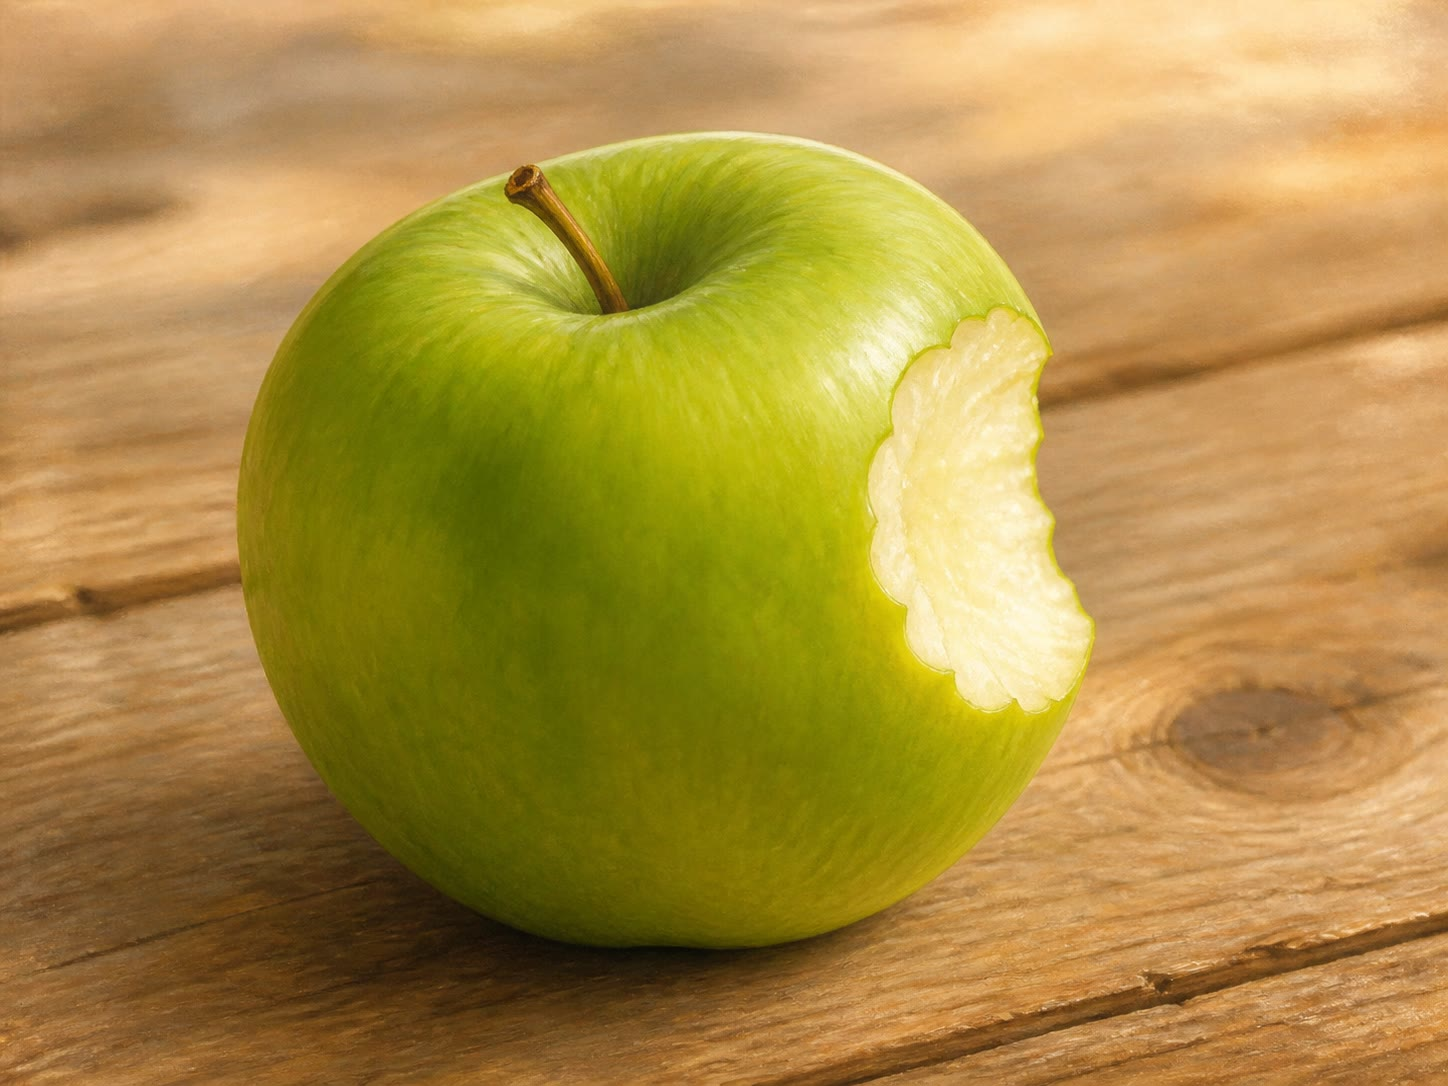
\includegraphics[width=0.55\linewidth]{images/book1/ai/g2-teeth-apple.jpg}

{\small Het eerste bewijsstuk van dit hoofdstuk: één hap, en de nette
gebogen handtekening van de \omterm{def:g2:teeth-and-eating-well:kinds}{snijtanden}.}
\end{omfigure}

\section{De tanden: een gereedschapskist in de mond}

\begin{definition}[De drie soorten tanden]\label{def:g2:teeth-and-eating-well:kinds}
Mensentanden bestaan in drie soorten, elk met een eigen taak:
\begin{enumerate}
  \item de \emph{snijtanden}\index{snijtand}, plat en scherp vooraan,
        \emph{snijden} --- ze snijden in de appel;
  \item de \emph{hoektanden}\index{hoektand}, puntig, in de hoeken,
        \emph{scheuren} --- ze grijpen taaier voedsel vast en trekken eraan;
  \item de \emph{kiezen}\index{kies}, breed en met knobbels achterin,
        \emph{vermalen} --- ze pletten het voedsel tot een brij die
        klaar is om door te slikken.
\end{enumerate}
\end{definition}

\begin{omfigure}
\begin{tikzpicture}
  \node[anchor=south west, inner sep=0] (img) at (0,0)
    {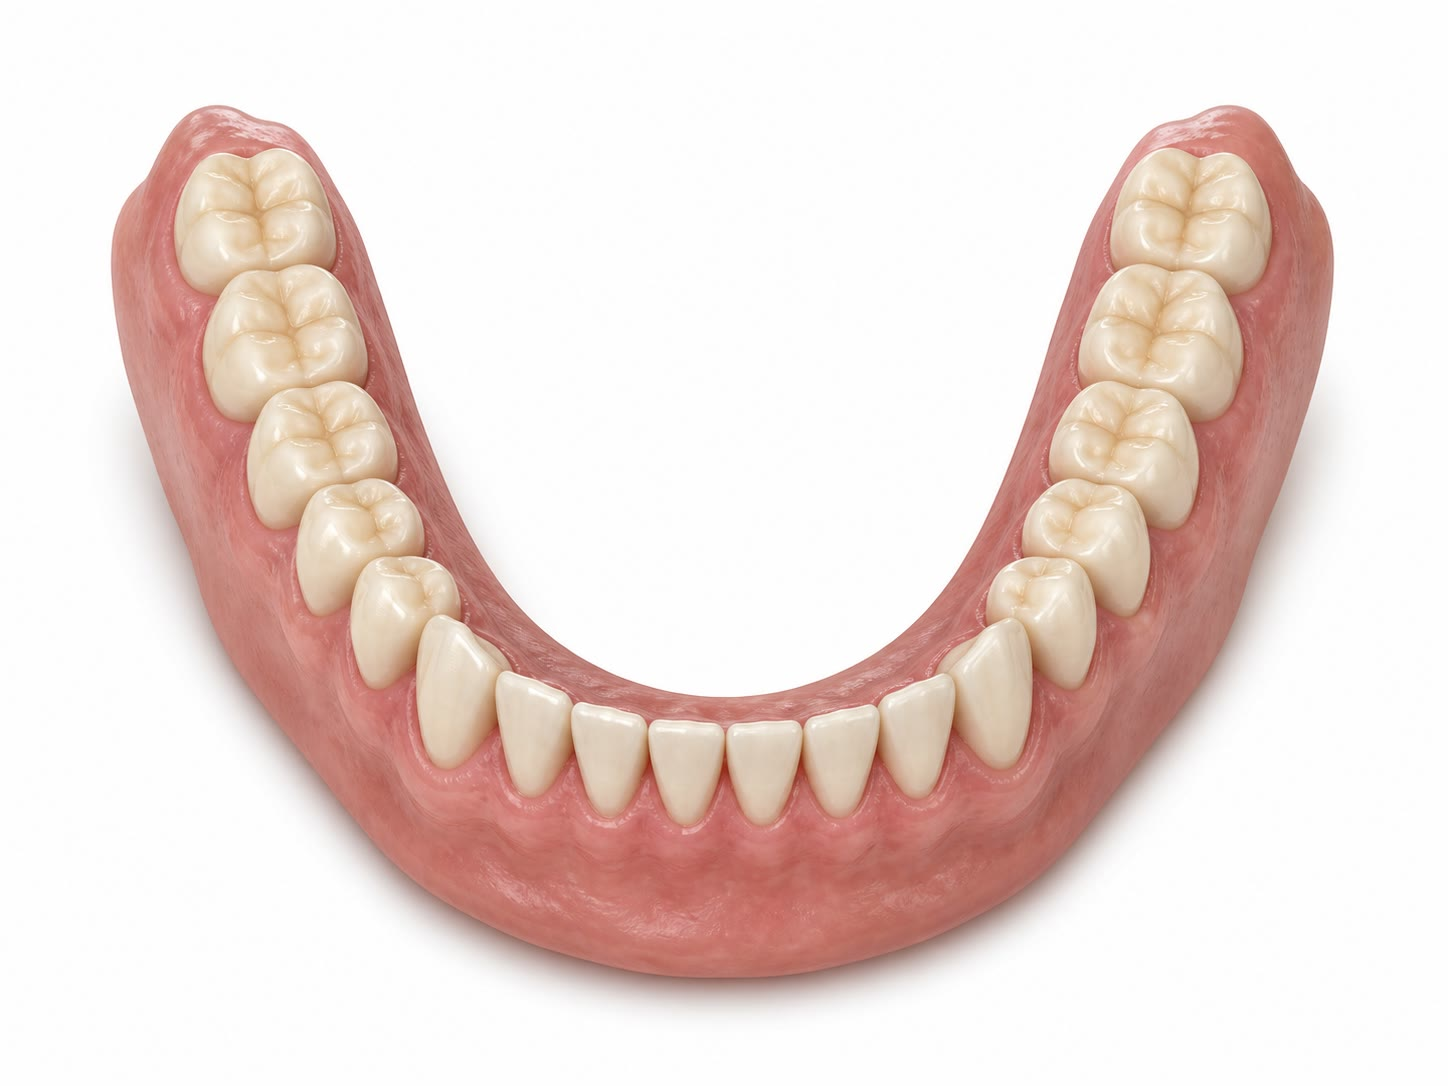
\includegraphics[width=0.56\linewidth]{images/book1/ai/fig-jaw-teeth.jpg}};
  \begin{scope}[x={(img.south east)}, y={(img.north west)},
      every node/.style={font=\small}]
    \draw[omDef, thick] (0.50,0.28) -- (0.50,0.06)
      node[below] {snijtanden: snijden};
    \draw[omThm, thick] (0.31,0.44) -- (-0.03,0.40)
      node[left, align=right, omThm] {hoektanden:\\ scheuren};
    \draw[omMeth, thick] (0.80,0.72) -- (1.03,0.72)
      node[right, align=left, omMeth] {kiezen:\\ vermalen};
  \end{scope}
\end{tikzpicture}

{\small De onderkaak: snijdende \omterm{def:g2:teeth-and-eating-well:kinds}{snijtanden} vooraan, scheurende
\omterm{def:g2:teeth-and-eating-well:kinds}{hoektanden} in de hoeken, malende kiezen achterin.}
\end{omfigure}

\begin{example}[Eén hap appel, drie gereedschappen]\label{ex:g2:teeth-and-eating-well:apple}
Een stuk appel eten gebruikt de hele gereedschapskist op volgorde: de
\omterm{def:g2:teeth-and-eating-well:kinds}{snijtanden} snijden de hap eraf, de \omterm{def:g2:teeth-and-eating-well:kinds}{hoektanden} helpen hem lostrekken, en
de \omterm{def:g1:the-five-senses:sense}{tong} schuift hem naar achteren naar de kiezen, die hem vermalen. Pas
daarna slik je.
\end{example}

\begin{remark}[Denk aan de dieren]\label{rem:g2:teeth-and-eating-well:animals}
Je gemengde gereedschapskist vertelt een verhaal: platte snijders en
maalkiezen als een \omterm{def:g2:what-animals-eat:kinds}{planteneter}, puntige \omterm{def:g2:teeth-and-eating-well:kinds}{hoektanden} als een \omterm{def:g2:what-animals-eat:kinds}{vleeseter}.
Het is de mond van een \omterm{def:g2:what-animals-eat:kinds}{alleseter} --- mensen zijn uitgerust voor \omterm{def:g1:plants-around-us:plant}{planten}
\emph{en} vlees, precies zoals \cref{ch:g2:what-animals-eat} ons indeelde.
\end{remark}

\section{Melktanden, blijvende tanden}

\begin{proposition}[Twee gebitten in één leven]\label{prop:g2:teeth-and-eating-well:sets}
Mensen krijgen twee gebitten. De $20$ \emph{melktanden}\index{melktand}
komen in de eerste levensjaren. Vanaf ongeveer zes jaar gaan ze wiebelen
en vallen ze een voor een uit, van onderaf weggeduwd door de
\emph{blijvende tanden}\index{blijvend gebit} --- het laatste gebit,
tot $32$ stuks, dat de rest van je leven mee moet.
\end{proposition}
\admitted

\begin{example}[De wiebelende snijtand]\label{ex:g2:teeth-and-eating-well:wobbly}
Een voortand begint precies te wiebelen op de leeftijd waarop kinderen
naar school gaan. Eronder is in alle stilte een blijvende \omterm{def:g2:teeth-and-eating-well:kinds}{snijtand}
gegroeid, die de \omterm{def:g1:plants-around-us:parts}{wortel} van de melktand heeft opgelost, tot het kleine
tandje loslaat. Het gat is geen ongelukje --- het is een wisseling.
\end{example}

\begin{remark}[Geen derde gebit]\label{rem:g2:teeth-and-eating-well:nothird}
Na het blijvende gebit komen er nooit meer nieuwe tanden. Een verloren
melktand wordt vervangen; een verloren blijvende tand is verloren. Dat
is de echte reden waarom volwassenen op poetsen staan: de tweede
gereedschapskist moet zeventig jaar of langer mee.
\end{remark}

\section{Goed eten}

\begin{proposition}[Een evenwichtig bord]\label{prop:g2:teeth-and-eating-well:balanced}
Om te groeien en gezond te blijven heeft het lichaam elke dag voedsel
uit elke familie nodig:
\begin{itemize}
  \item groente en fruit --- voor de vitamines, bij elke maaltijd;
  \item brood, granen, aardappelen --- voor langdurige energie;
  \item \omterm{def:g2:animals-grow-up:born}{melk}, yoghurt, kaas --- om botten en tanden mee te bouwen;
  \item vlees, vis of eieren --- om het lichaam mee te bouwen, een of
        twee keer per dag is genoeg;
  \item water --- de enige drank die het lichaam echt nodig heeft;
  \item zoete en vette lekkernijen --- voor het plezier, in kleine
        hoeveelheden, niet bij elke maaltijd.
\end{itemize}
\end{proposition}
\admitted

\begin{example}[Twee tussendoortjes]\label{ex:g2:teeth-and-eating-well:snack}
Als tussendoortje A: een appel, een boterham en wat water. En als
tussendoortje B: snoep en een frisdrank. B smaakt naar suiker en verder
naar weinig --- en suiker is precies waar de \omterm{def:g1:healthy-habits:germs}{ziektekiemen} uit
\cref{ch:g1:healthy-habits} van smullen. Tussendoortje A voedt het
lichaam en geeft de tanden eerlijk werk. Raad eens welke de tandarts
voor haar eigen kinderen inpakt.
\end{example}

\begin{method}[Een dagmenu nakijken]\label{met:g2:teeth-and-eating-well:check}
Neem de maaltijden van een dag en kijk na:
\begin{enumerate}
  \item groente of fruit bij elke maaltijd?
  \item iets uit de bouwfamilies --- zuivel, en vlees, vis of eieren?
  \item water als dagelijkse drank?
  \item lekkernijen klein en af en toe gehouden?
\end{enumerate}
Als er een familie ontbreekt, is de volgende maaltijd de kans om haar
weer uit te nodigen.
\end{method}

\section{Oefeningen}

\begin{exercise}[$\star$]\label{exo:g2:teeth-and-eating-well:1}
Noem de drie soorten tanden en de taak van elk.
\end{exercise}

\begin{exercise}[$\star$]\label{exo:g2:teeth-and-eating-well:2}
Welke tanden zitten vooraan in de mond, en welke achterin?
\end{exercise}

\begin{exercise}[$\star$]\label{exo:g2:teeth-and-eating-well:3}
Volg een hap \omterm{def:g1:plants-around-us:parts}{wortel} door de mond: welke tand doet wat, en in welke volgorde?
\end{exercise}

\begin{exercise}[$\star$]\label{exo:g2:teeth-and-eating-well:4}
Hoeveel \omterm{prop:g2:teeth-and-eating-well:sets}{melktanden} zijn er? Wat gebeurt er met ze vanaf ongeveer zes jaar?
\end{exercise}

\begin{exercise}[$\star$]\label{exo:g2:teeth-and-eating-well:5}
Waarom moeten \omterm{prop:g2:teeth-and-eating-well:sets}{blijvende tanden} nog beter verzorgd worden dan \omterm{prop:g2:teeth-and-eating-well:sets}{melktanden}?
\end{exercise}

\begin{exercise}[$\star$]\label{exo:g2:teeth-and-eating-well:6}
Noem de voedselfamilies die op een gezonde dag horen. Welke drank heeft
het lichaam echt nodig?
\end{exercise}

\begin{exercise}[$\star$]\label{exo:g2:teeth-and-eating-well:7}
Vergelijk de twee tussendoortjes uit \cref{ex:g2:teeth-and-eating-well:snack}:
wat geeft tussendoortje A het lichaam dat tussendoortje B niet geeft?
\end{exercise}

\begin{exercise}[$\star$]\label{exo:g2:teeth-and-eating-well:8}
Probeer het: bekijk je eigen tanden in een spiegel. Zoek een \omterm{def:g2:teeth-and-eating-well:kinds}{snijtand},
een \omterm{def:g2:teeth-and-eating-well:kinds}{hoektand} en een kies, en vergelijk hun vorm met de figuur.
\end{exercise}

\begin{exercise}[$\star\star$]\label{exo:g2:teeth-and-eating-well:9}
Leg met \cref{rem:g2:teeth-and-eating-well:animals} uit wat de vorm van
mensentanden over het menselijke menu zegt --- en op welke \omterm{def:g1:animals-around-us:animal}{dieren} uit
\cref{ch:g2:what-animals-eat} we lijken.
\end{exercise}

\begin{exercise}[$\star\star$]\label{exo:g2:teeth-and-eating-well:10}
De dag van Lila: ontbijt --- ontbijtgranen met \omterm{def:g2:animals-grow-up:born}{melk}; lunch --- pasta en
snoep; tussendoortje --- frisdrank en koekjes; avondeten --- pizza.
Laat \cref{met:g2:teeth-and-eating-well:check} erover lopen: wat
ontbreekt, en wat komt er te vaak voor?
\end{exercise}
